\documentclass[a4paper]{article}

\usepackage[english]{babel}
\usepackage[utf8]{inputenc}
\usepackage{amsmath}
\usepackage{graphicx}
\usepackage[colorinlistoftodos]{todonotes}
\usepackage{verbatim}
\usepackage{tikz}
\usepackage{array}
\def\checkmark{\tikz\fill[scale=0.4](0,.35) -- (.25,0) -- (1,.7) -- (.25,.15) -- cycle;} 

\title{Small Project Proposal Virtual Reality Museum}

\author{Bibi de Boer \and Wouter Florijn \and Xhi Jia Tan}

\date{\today}

\begin{document}
\maketitle

\section{Introduction}

Virtual Reality (VR) is defined by Merriam-Webster \cite{merriam} as \emph{an artificial world that consists of images and sounds created by a computer and that is affected by the actions of a person who is experiencing it}. The artificial world can either be a representation of the real world, or an imaginary world \cite{martens}. VR systems in the past were relatively specialized systems with not many users \cite{martens}. In 2012, Oculus created a Kickstarter \cite{kickstarter} for the Rift \cite{oculus}, a virtual reality headset. The project was funded and  introduced virtual reality to a more general public. As VR became more widely used, larger companies such as Samsung and Google developed their own VR variants \cite{gearvr, cardboard}, enabling the use of VR on mobile devices. 

VR can be applied in different domains, including those which do not have a direct association with computer technology. One of such domains is cultural heritage \cite{wojciechowski}, and more specifically, museums. This research will be focused on virtual museums. Work in this domain has focused mainly on realistic recreation of existing museums and collections. However, VR provides many possibilities beyond this purpose. Using VR, scenarios could be created that would be impractical or even impossible to create in the real world. Therefore, this research will look beyond simply replicating museums, and will aim to find new ways of improving the user experience by using illusions in VR to alter the surroundings of a painting in a virtual museum setting.


\subsection{Virtual Museums}
Many connections have been made between museums and the virtual  world. For example, the famous Louvre museum provides virtual tours consisting of 360 degrees pictures through which you can navigate \cite{louvre}. This gives people a chance to 'visit' the museum without physically being there. Instead of using pictures, Wojciechowski et al. \cite{wojciechowski} developed the ARCO system that provides museums tools to build and manage their Virtual and Augmented reality exhibitions. Using the ARCO system, Whole virtual museums can be built. This enables museums to show pieces for which they do not have the physical space. 

The creation of a virtual space can even be taken a step further by creating a whole different virtual scene. The Westfries museum in Hoorn in the Netherlands has created a VR experience \cite{westfries} as a piece of their exhibition, allowing visitors to relive Hoorn in the Dutch Golden Age.
These projects on the domain of VR in cultural heritage focus on imitating the original environment, or on creating a new environment which portrays the environment like it was historically.

\subsection{Altering the Environment of Paintings}

%\textbf{A section about a paper about regular virtual museums has to be inserted here, but we have not read a suitable paper yet. This needs to bridge the gap between the previously mentioned VR museums and exhibitions of paintings.}

The traditional setup of a quiet white room is not the only way to display paintings. The Tate Sensorium \cite{tate1} in Tate Britain added touch, taste, smell and sound in their galleries \cite{tate2}. The setting of the painting was modified by adding more modalities to change the way viewers perceive it. Using VR, these modalities can also be used, without the need to adapt the physical environment. This project however does not have the goal to imitate the Tate Sensorium in the VR space. Instead, it will make use of a different sense, vision, to enhance the experience of viewing paintings.

The IllumiRoom system \cite{illumiroom} enhances the experience of playing a game or watching a movie by projecting additional information around the high resolution display, in the peripheral view of the user. Various illusions are discussed in the paper, all of which add extra context based on events occurring on the display. The IllumiRoom system augments the physical surroundings of the player to create a better gaming experience. In the IllumiRoom system, this augmenting feature is used with games to create a better gaming experience. However, changing the surrounding can also be done for other objects of interest. In our case, the environment of paintings will be changed in order to create a different experience while viewing them.

% IllumiRoom references: [18, 14, 13, 29, 1]
%need more directly related work: ambilight


A museum usually provides different types of exhibitions pieces. This project will focus on paintings as exhibition pieces, and like the Tate Sensorium \cite{tate2}, changing the perception of the paintings. It will lend the idea of the IllumiRoom system \cite{illumiroom} by changing the visual surroundings of a painting to enhance the user experience when watching a painting. 



% why it should be implemented in a vr museum and not in a real museum. NOT why we use vr. Let's assume our focus is to create a better experience in VR museums, which might spark interest in real museums.
The environment of the paintings is changed by adding illusions. They can for example consist of creating new objects or showing animations. These illusions are not simple to realize in physical museums. Especially animated illusions are difficult to create in galleries without the necessary equipment. Projectors can be used to project animations on the walls, but this would result in shadows when people are walking by. The room would also have to be dark in order to make the projection properly visible. Large displays can be used to avoid these issues. However, these screens require a considerable amount of money. 

Finally, using VR allows us to create a unique experience for each user, as opposed to having them all see the exact same thing. For these reasons, VR museums are a more suitable medium for the realization of these illusions. Additionally, the benefits and novelty of VR could create a stimulating effect for people who otherwise would not visit museums, which could eventually generate interest in museums in general.

\section{Research Goal}
The goal of this research is to find ways of improving the user experience in a virtual museum setting. While there are various types of museums, we focus on exhibitions of paintings in particular. Since paintings can be displayed as 2D images, various image processing techniques can be applied to them, which are useful for some of our methods. Visible alterations are used to change the environment of the paintings. We aim to find interesting illusions that could be applied in various applications related to virtual museums. As it is a big part of user experience, we look into the enjoyment a user experiences when looking at paintings in the altered environment. This might open up new possibilities and ideas for creating new virtual museums and possibly spark interest in those who are normally not interested in visiting museums.

\subsection {Research Questions}

As indicated by our research goal, we want to make viewing paintings more enjoyable for people who would normally not enjoy viewing paintings very much by visually altering the environment of the painting. We call these alterations 'illusions'. We aim to answer the following question:
\begin{itemize}
\item{\emph{How do illusions affect the enjoyment of viewing a painting in a VR museum setting?}}
\end{itemize}
The illusions will be defined and explained in section \ref{design space}. 

In this research, the enjoyment of the user is seen as a big part of the user experience. As the virtual museum is a VR experience, the user's sense of presence, the feeling of being in the virtual world, might influence the level of enjoyment. These two metrics have been shown to be connected in related applications \cite{sylaiou}. This is a strong indication that enjoyment is influenced by presence in the context of virtual museums, and thus in the context of our research. Therefore, measuring the presence is essential, as it influences enjoyment in a VR setting. Enjoyment is measured to get an indication of positive user experience. This results in the subquestion:

\begin{itemize}
\item{\emph{How do the illusions influence the sense of presence in the world of the virtual museum?}}
\end{itemize}

Besides the sense of presence and enjoyment the user experiences in the virtual world, it is also important to look at the user’s connection to the painting specifically. With the illusions, we aim to create a stronger connection between the user and the painting by extending characteristics of the painting beyond its frame. We aim to make the user feel more like he is part of the world of the painting, than of the world of the museum. This type of connection can be seen as another layer of presence in a virtual world; the presence in the world of the painting. We will refer to this type of presence as connectedness, and ask the following subquestion:

\begin{itemize}
\item{\emph{How do the illusions influence the sense of connectedness to the painting?}}
\end{itemize}

Furthermore, we are interested in whether or not the illusions can generate more interest in art for people who are generally not interested in visiting museums. For this we want to know if the illusions create more interest to users compared to the VR museum settings without illusions. One indication for interest would be the duration people look at the painting directly, versus how much time they spent looking at the illusion. Additionally, users can be asked about their willingness to visit an art museum before and after using our VR application. This gives raise to the following subquestions:

\begin{itemize}
\item{\emph{How do the illusions influence the interest in the painting?}}
\item{\emph{How do the illusions influence willingness to visit art museums?}}
%mss overbodig... point of interest vertelt niet hoe iemand "meer" geinteresseerd is
%\item{\emph{What part of the setting is the center point of attention?}}
\end{itemize}

\section{Design Space}\label{design space}

There are lots of ways to alter the surroundings of the painting that could potentially enhance the experience of looking at a painting, and make it more interesting. For example, the color of the walls can be changed depending on the painting, or an image can be used to decorate the walls, instead of having a regular wall that is painted in one color. A few more examples of these illusions with their details will be given in sections \ref{sec:stateffects} and \ref{sec:animeffects}. There are also many possiblitities for the space of the room where the illusion is displayed. Those are described in section \ref{sec:spaceinroom}. 

\subsection{Space in the room}\label{sec:spaceinroom}
Like in \cite{illumiroom}, there are many possible locations to project the illusions in this application. Listed here some of the possible spaces of the room that can be utilized by these illusions:

\begin{comment}
\begin{table}
\begin{tabular}{ | p{5.5cm} | p{5.7cm} | }
\hline
\textbf{Only affects wall behind painting} & \textbf{Affects entire room} \\\hline
Changing or static color on the wall & On all walls \\\hline
Picture in genre of painting & \\\hline
Video in genre of painting & \\\hline
Picture in the style of the painting & Current camera image in the style of the painting \\\hline
Wall in style of the painting & Room in style of the painting (altered 3D models or just altered textures) \\\hline
Extended painting & Extend the painting over all textures in the room \\\hline
IllumiRoom 'weather illusion' on wall & Moving freely through the room  \\\hline
\end{tabular}
\caption{Some illusions that can be applied to a museum room in VR}
\label{tab:effect_ideas}
\end{table}
\end{comment}

\begin{itemize}
\item Affecting the walls
\begin{itemize}
\item Directly around the painting
\item The entire wall behind the painting
\item Multiple walls
\end{itemize}
\item Affecting the 3D space of the room
\begin{itemize}
\item A specific area
\item The entire 3D space
\end{itemize}
\end{itemize}

%For this research, only illusions affecting the whole wall and the 3D space will be used. The reason for this is to test if the illusions work when fully applied compared to no illusions at all. This way making decisions about the size of the area influenced by the illusions can be avoided.

For this research, only illusions affecting the entire 3D space or the entire wall behind the painting will be considered. Since there are infinitely many ways of designing and partitioning a room, this decision is necessary to reduce the design space to a feasible number of possibilities. 

\subsection {Types of illusions}
Besides the shape and location of the illusions, we can also distinguish between static and animated illusions. We will describe these categories of illusions in sections \ref{sec:stateffects} and \ref{sec:animeffects} respectively.

\subsubsection{Static Illusions}\label{sec:stateffects}

In this subsection we will discuss the part of the design space consisting of static illusions. These illusions will alter the surroundings of the painting without the use of animations. This will serve as an introduction to the animated illusions, which will be discussed in section \ref{sec:animeffects}.
%In this section we will give examples of static effects to change the surroundings of a painting. %We will then go into more detail about the illusions we will use in section \ref{sec:animeffects}.

\begin{itemize}

\item{\textbf{Static color on the wall}} %Try to find some exhibition guideline research about backgrounds (colors) to paintings 
\\One of the most basic things to do to change the direct environment of a painting is to simply paint the wall in a color that makes the painting stand out better. The best color is a color that the user does not notice and where he only remembers the colors of the painting \cite{colorwall}. These colors could also affect the ambiance of the room and the mood of the person\cite{mood} viewing the painting. This illusion could affect only the whole wall the painting is hanging from, or the entire room.

\item{\textbf{Picture of a subject related to the painting}} 
\\Another change would be to decorate the wall with a picture. Sometimes, when displaying a collection of pictures or drawings, a museum shows one of the images on the back wall behind the frames (fig \ref{fig:picturewall}).

\begin{figure}[h!]
\label{fig:picturewall}
\centering
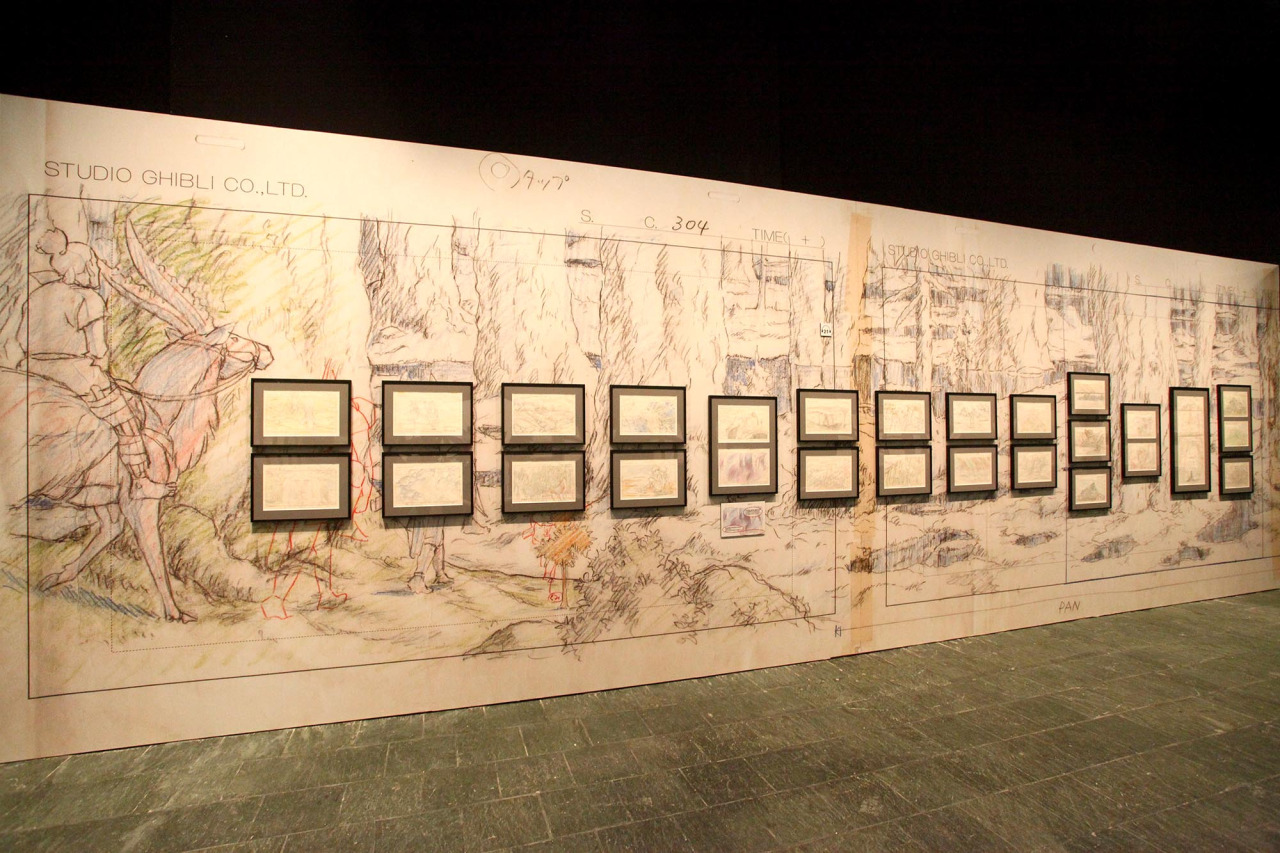
\includegraphics[width = 90mm]{PictureWall.jpg}
\caption{An exhibition piece used as wall image at the Studio Ghibli Layout Designs exhibition in the Hong Kong Heritage Museum}
\end{figure}

\item{\textbf{Picture in style of the painting}}
\\In \cite{gatys}, a picture is altered to be stylized in the same way as a painting is. An image is produced that still shows the content of the picture, but it appears to be painted in the same style as the painting. Instead of using a regular picture as in the example above, the picture could be processed to get the same style as the painting. That picture can then be displayed on the wall behind the painting. This could make for a better backdrop to the painting than a regular picture would, as it better resembles the painting. Since the algorithm can be applied to any type of image, three different ways of applying it in our museum setting come to mind. 

Firstly, the style of the painting could simply be applied to a single object in the environment, such as a picture projected on a wall. This could easily be done using preprocessing. 

Secondly, the style could be applied as a post-processing effect to the user's field of view. Each frame the user sees through the VR device will be processed to have the same style as the painting. However, some issues can be foreseen with this type of application, as processing might take too long to maintain a decent framerate. Additionally, a very subtle change in head orientation could cause a very large change in the rendered view, as the entire frame would have to go through the process again. 

Finally, we can apply the style of the painting to the textures of all objects in the room. This way we can take advantage of preprocessing and therefore avoid the drawbacks of the previous method. A possible downside however, is that the illusion would only be applied to textures and therefore would not affect 3D shapes and shadows.

\item{\textbf{Extending the painting}}
\\If a painting is a window into the world of the painter, then what is behind that museum wall? With a method called inpainting \cite{inpainting}, it is possible to extrapolate information from the painting and apply it to the empty wall surrounding it. In this way, the wall can be made to look like an extension of the painting - like the wall and the painting are actually one big painting.

\end{itemize}

\subsubsection{Animated Illusions}\label{sec:animeffects}

Some illusions mentioned in the previous section can also have an animated variant and some illusions can only be achieved when animated.

\begin{itemize}

\item{\textbf{Changing colors on the wall}}
\\In the virtual space, the wall would not need to be one color, but could change color over time to create different moods.

\item{\textbf{Video related to the painting}}
\\A video would be the more dynamic version of the still picture. For example, behind old news pictures, a news video covering the same event could be shown. The emphasis would still be on the pictures, and the video could intensify the experience by making the surroundings supplement the displayed art.

\item{\textbf{Picture in style of the painting}}
\\Another animated illusion uses a picture shown on the back wall, while the picture slowly morphs into the same style as the painting. In \cite{gatys}, the grade of stylization can be controlled. In this way, multiple images can be produced that are in style somewhere in between the unaltered picture and the style of the painting. With those, an animation can be made of the picture slowly changing to match the style of the painting.

\item{\textbf{Extending Painting}}
\\For this animated illusion, the painting expands over the back wall while the user is watching it. This can be done by using painting expansion software \cite{inpainting}. The wall around the painting is filled with textures extrapolated from the painting.


\item{\textbf{IllumiRoom 'weather illusions'}}
\\Lastly, the room or the walls can be filled with particles that relate in some way to the painting, like snowflakes for a snowy painting or leaves for a painting of a forest in fall. Instead of basing these illusions solely on weather, they can be generalized to various particle effects based on the setting of the painting. These illusions are based on the IllumiRoom \emph{Snow} illusion \cite{illumiroom} and are discussed in more detail in section \ref{sec:methods}.
\end{itemize}

\subsection{Utilized design space} 

For this research, the animated illusions of the stylized picture, extension of the painting and the IllumiRoom weather illusion appear to be the most promising to see as a visual effect. These illusions can be applied to almost any kind of painting and use modifications based directly on the painting. They can be customized extensively to fit the need of the user or curator, but also leave open the option of automatization. These illusions are very hard or even impossible to create in real museums. However, by utilizing the aspects of virtual reality, these illusions can be created in a virtual museum.

Not every type of illusion is suitable to be applied on both the wall around the painting as well as in the 3D space. The same can be said about whether these illusions only have an animated version, or a static version as well. In table \ref{tab:ourillusions}, the suitable combinations that are going to be tested can be found. 

\begin{table}
\centering
\begin{tabular}{ | l | >{\centering}p{1.7cm} >{\centering}p{1.7cm} | >{\centering}p{1.7cm} c | }
\hline
 & Wall space & 3D space & Static & Animated \\\hline
Stylized & $\surd$ &  & $\surd$ & $\surd$ \\
Extended & $\surd$ &  & $\surd$ & $\surd$ \\
Weather & $\surd$ & $\surd$ &  & $\surd$ \\\hline
\end{tabular}
\caption{\label{tab:ourillusions}The illusions used in this research and their tested spaces in the room}
\end{table}

\begin{comment}
\section{Research Goal}
The goal of this research is to find ways of improving the user experience in a virtual museum setting. We aim to find interesting visual effects that could be applied in various applications related to virtual museums. We hope this will open up new possibilities of getting people who are not interested in visiting museums more interested in art by offering them a unique and accessible way to explore art collections.

\subsection {Research Questions}
We would like to investigate whether the chosen illusions affect the experience of viewing a painting, and whether they affect the duration the viewer looks at the painting. We want to know which illusion enhances the experience the most.

\emph{How do visual illusions affect the experience of viewing a painting in a VR setting?}

The three animated illusions will be compared with a museum room without any illusions. A user study will be conducted to research how the illusions change the experience of looking at a painting in a museum. 
We want to measure how interesting and enjoyable these settings are to look at. We are particularly interested in whether or not the illusions can generate more interest in art in people who are generally not interested in visiting museums.
We are also interested in what they find most interesting to look at - are they more interested in the painting itself, or in our illusions? Are they comparing, looking to and from the painting and its background (or foreground, in case of the weather illusions). Are people still looking at the painting with so much going on around it? We ask two subquestions which will contribute to answering our main research question.

\emph{How do the illusions influence the enjoyment of viewing a painting?}

\emph{What part of the setting is the center point of attention?}
\end{comment}

\section{Methods} \label{sec:methods}

The application will be implemented using Google Cardboard. Google Cardboard is a VR device that uses a smartphone as a display. This device has the benefit of being cheap, portable and easy to use, making it easily accessible to museums or individuals.

%uitleg nodig dat 12 paintings voldoende is om te generaliseren?
To answer our research questions, we will implement various illusions for different paintings and use them to conduct a user study. Paintings with three different types of content, painted in two different artistic styles will be used. For each combination, two different paintings will be selected as a representation. This means that we will use a total of twelve different paintings. In order to achieve reliable results, the paintings used will be carefully selected, so that they provide a good representation of a large collection of paintings. The selected paintings can be found in appendix~\ref{sec:paintings}. Even though this will likely not be sufficient to represent all paintings, with this selection, we aim to provide a fair sample of a vast group of paintings they belong to.

For the content we will use the following categories:

\begin{itemize}
\item \textbf{Forests.} Paintings of forests, depicting trees and other foliage.
\item \textbf{Seascapes.} Paintings of open sea or seashores containing both sea and land.
\item \textbf{Snowy environments.} Paintings of landscapes covered in snow, paintings where snow is falling.
\end{itemize}

We have chosen these categories because they are general enough to represent a large subgroup of all paintings, yet they are easy to distinguish between because of their well-defined characteristics.

We will use the following artistic styles:

\begin{itemize}
\item \textbf{Photorealistic paintings.} Paintings depicting the content in an accurate and realistic way.
\item \textbf{Stylized paintings.} Paintings depicting the content with a distinctive style, like coarse brush strokes.
\end{itemize}

We have chosen these two different styles to be able to investigate the effects of the illusions for different types of paintings. If an illusion works well for a photorealistic painting, this doesn't imply it also works well for a stylized painting.

As discussed in section \ref{sec:animeffects}, we will apply the following three animated illusions for each painting:

\begin{itemize}
\item \textbf{Stylized picture.} For this illusion we will overlay a picture on the wall behind the painting. The style of the painting will be applied to the picture using methods described in \cite{gatys}. Pictures will be different for each painting and will be selected to have content similar to the painting. This illusion will be used as animation as well as static.
\item \textbf{Extending the painting.} For this illusion we will display content based on the painting on the wall behind it \cite{inpainting}. This illusion will be used as animation as well as static.
\item \textbf{Weather-like effects.} For this illusion we will create 3D particles or objects based on the weather conditions and content of the painting. These particles will include snow, rain or falling leaves. This illusion will be tested both when displayed on the wall behind the painting, as in the 3D space of the room.
\end{itemize}

\subsection{Experiment Setup}

The animated illusions can be implemented in various ways, including different values for parameters such as speed or behaviors of animation. To get a set value for these settings, a pre-experiment will be done to find the most promising settings in terms of enjoyment and presence. This can first be done internally and then tested on three to five people, giving their opinion about the different settings of the illusions. These participants are not allowed to join the main experiment anymore as they have seen the illusions before. This can influence their final judgment.

For the main experiment, participants will be subdivided into four groups. These groups consist of at least twenty participants. We will have one group for each illusion, and one control group to which a default museum room will be presented. Each group will look at each of the twelve paintings. 
For each participant, the environment for the twelve settings will be similar. Every time they will be placed in a room based on a part of a museum. The room will contain one painting and will have some additional objects such as chairs or plants. These objects will be used to facilitate features of various illusions. Apart from this, the room will be fairly plain in order to avoid distraction.

The first three groups will each have an illusion applied during the tests. Each of these groups will be presented with one of the three illusions discussed above. The fourth group will simply be placed inside the default room with no illusion applied. 

Before and after a participant has finished the tests, he will fill out a questionnaire. The before-questionnaire will be shorter.

\subsubsection{Measurements}\label{sec:measurements}

The user will first be interviewed about their interest in art and willingness to visit art museums by means of a questionnaire. This questionnaire will then be repeated after the experiment so see whether their opinion has changed.

Using a questionnaire, we intend to capture the user's sense of presence and enjoyment. This survey will be an adapted and combined version of the presence questionnaire by Witmer \& Singer \cite{witmer} and The Groningen Enjoyment Questionnaire \cite{stevens}.

To measure the participants' interest in the painting and the illusion, the direction in which they are looking will be tracked during the experiment. The amount of time the participants are looking directly at the painting or at the illusion will be measured in order to determine whether or not the environment draws away the user's attention from the painting. 

The measured variables will be statistically analyzed. We will compare the results of all groups to determine the difference between each illusion and the default case. Our results will show the differences in terms of interest, presence and enjoyment for each combination of groups. These results will grant insight into the impact of the different illusions.

\subsection{Analysis}
To Be Decided.

\section {Hypothesis \& Conclusion}
We expect that every illusion will captivate users more than a regular painting in a white room would, causing them to use the application for a longer period of time. Adding these illusions will create a new virtual museum experience, that might pique the curiosity of those who are normally not interested in museums. They might take the virtual museum tour for the illusions, and will then be exposed to the paintings nevertheless, providing a chance to raise their interest in art. 

This research will help expand the world of digital museums. In virtual reality, not everything has to behave like it would in the real world. This research explores and tries to expand the borders of virtual museums by adding illusions that would be impractical without the use of VR. This specific area is largely unexplored. Research in this area could open up a lot of possibilities.

Real life museums could make their exhibits more interesting to people who would normally not visit them. This research could tell them what kind of illusion would be interesting to those people. These people could then look at the paintings through an Augmented Reality headset, or through the camera of their smartphone, while the regular visitors can still enjoy the painting on the background of a bland wall. Alternatively, they could visit parts of the museum in VR, and visit the real museum afterwards.



\begin{thebibliography}{99}

\bibitem{merriam} Merriam-Webster:
\emph{Dictionary}
Web [Last accessed on October 19, 2015]
http://www.merriam-webster.com/dictionary/virtual\%20reality

\bibitem{martens} Jon Martens \& Pavlo D. Antonenko:
\emph{Narrowing gender-based performance gaps in virtual environment navigation},
Computers in Human Behavior 28, p 809-819, 2012

\bibitem{kickstarter}
\emph{Oculus Rift: Step Into the Game}
Web [Last accessed on November 5, 2015]
https://www.kickstarter.com/projects/1523379957/oculus-rift-step-into-the-game/description

\bibitem{oculus}
\emph{Rift}
Web [Last accessed on October 20, 2015]
https://www.oculus.com/ja/rift/

\bibitem{gearvr}
\emph{Samsung Gear VR}
Web [Last accessed on October 20, 2015]
http://www.samsung.com/global/microsite/gearvr/index.html


\bibitem{tate1}
\emph{IK Prize 2015: Tate Sensorium}
Web [Last accessed on November 5, 2015]
http://www.tate.org.uk/whats-on/tate-britain/display/ik-prize-2015-tate-sensorium

\bibitem{tate2}
\emph{Welcome to Tate Sensorium: taste, touch and smell art - video}, 
The Guardian,  25 August 2015.
Web [Last accessed on November 5, 2015]
http://www.theguardian.com/artanddesign/video/2015/aug/25/welcome-tate-sensorium-taste-touch-smell-art-video


\bibitem{cardboard}
\emph{Google Cardboard}
Web [Last accessed on October 20, 2015]
https://www.google.com/get/cardboard/

\bibitem{wojciechowski} Rafal Wojcieshowksi, Krzysztof Walczak, Martin White \& Wojcieh Cellary
\emph{Building Virtual and Augmented Reality museum exhibitions},
The Poznan University of Economics, Poland,
University of Sussex, UK, 2014

\bibitem{westfries}
\emph{Kaap Varen}
Web [Last accessed on October 19, 2015]
http://wfm.nl/kaap-varen/

\bibitem{louvre}
\emph{Online Tours}
Web [Last accessed on October 19, 2015]
http://www.louvre.fr/en/visites-en-ligne

\bibitem{gatys} Leon A. Gatys, Alexander S. Ecker \& Matthias Bethge:
\emph{A Neural Algorithm of Artistic Style},
CoRR, 2015

\bibitem{witmer} Bob G. Witmer \& Michael J. Singer:
\emph{Measuring Presence in Virtual Environments: A Presence Questionnaire},
U.S. Army Research Institute for the Behavioral and Social Sciences, 1994

\bibitem{stevens} Stevens et. al.:
\emph{The Groningen Enjoyment Questionnaire: A measure of enjoyment in leisure-time physical activity},
Perceptual and Motor Skills, 200

\bibitem{illumiroom} Brett R. Jones, Hrvoje Benko, Eyal Ofek, Andrew D. Wilson:
\emph{IllumiRoom: Peripheral Projected Illusions for
Interactive Experiences},
Proceedings of the SIGCHI Conference on Human Factors in Computing Systems, p 869-878, 2013

\bibitem{inpainting}
\emph{Extending Van Gogh’s \emph{Starry Night} with Inpainting}
Web [Last accessed on October 19, 2015]
http://blog.wolfram.com/2014/12/01/extending-van-goghs-starry-night-with-inpainting/

\bibitem{sylaiou} Sylaiou et. al.:
\emph{Exploring the relationship between presence and enjoyment in a virtual museum},
Int. J. Human-Computer Studies 68, 2010, pp. 243--253

\bibitem{mood}
\emph{Colour Theraphy}, 
The Guardian, 6 July 2008.
Web [Last accessed on November 5, 2015]
http://www.theguardian.com/lifeandstyle/2008/jul/06/healthandwellbeing.relaxation31

\bibitem{colorwall} Jonathan Jones
\emph{What colour should gallery walls be?}
The Guardian, 21 October 2011.
Web [Last accessed on November 11, 2015]
http://www.theguardian.com/artanddesign/jonathanjonesblog/2011/oct/21/colour-gallery-walls-musee-d-orsay


\end{thebibliography}











\newpage

\appendix
\section{Paintings} \label{sec:paintings}

\subsection{Forest}

\subsubsection{Realistic forest paintings}
\begin {figure}[h!]
\centering
\begin{minipage}[b]{.49\textwidth}
	\centering
	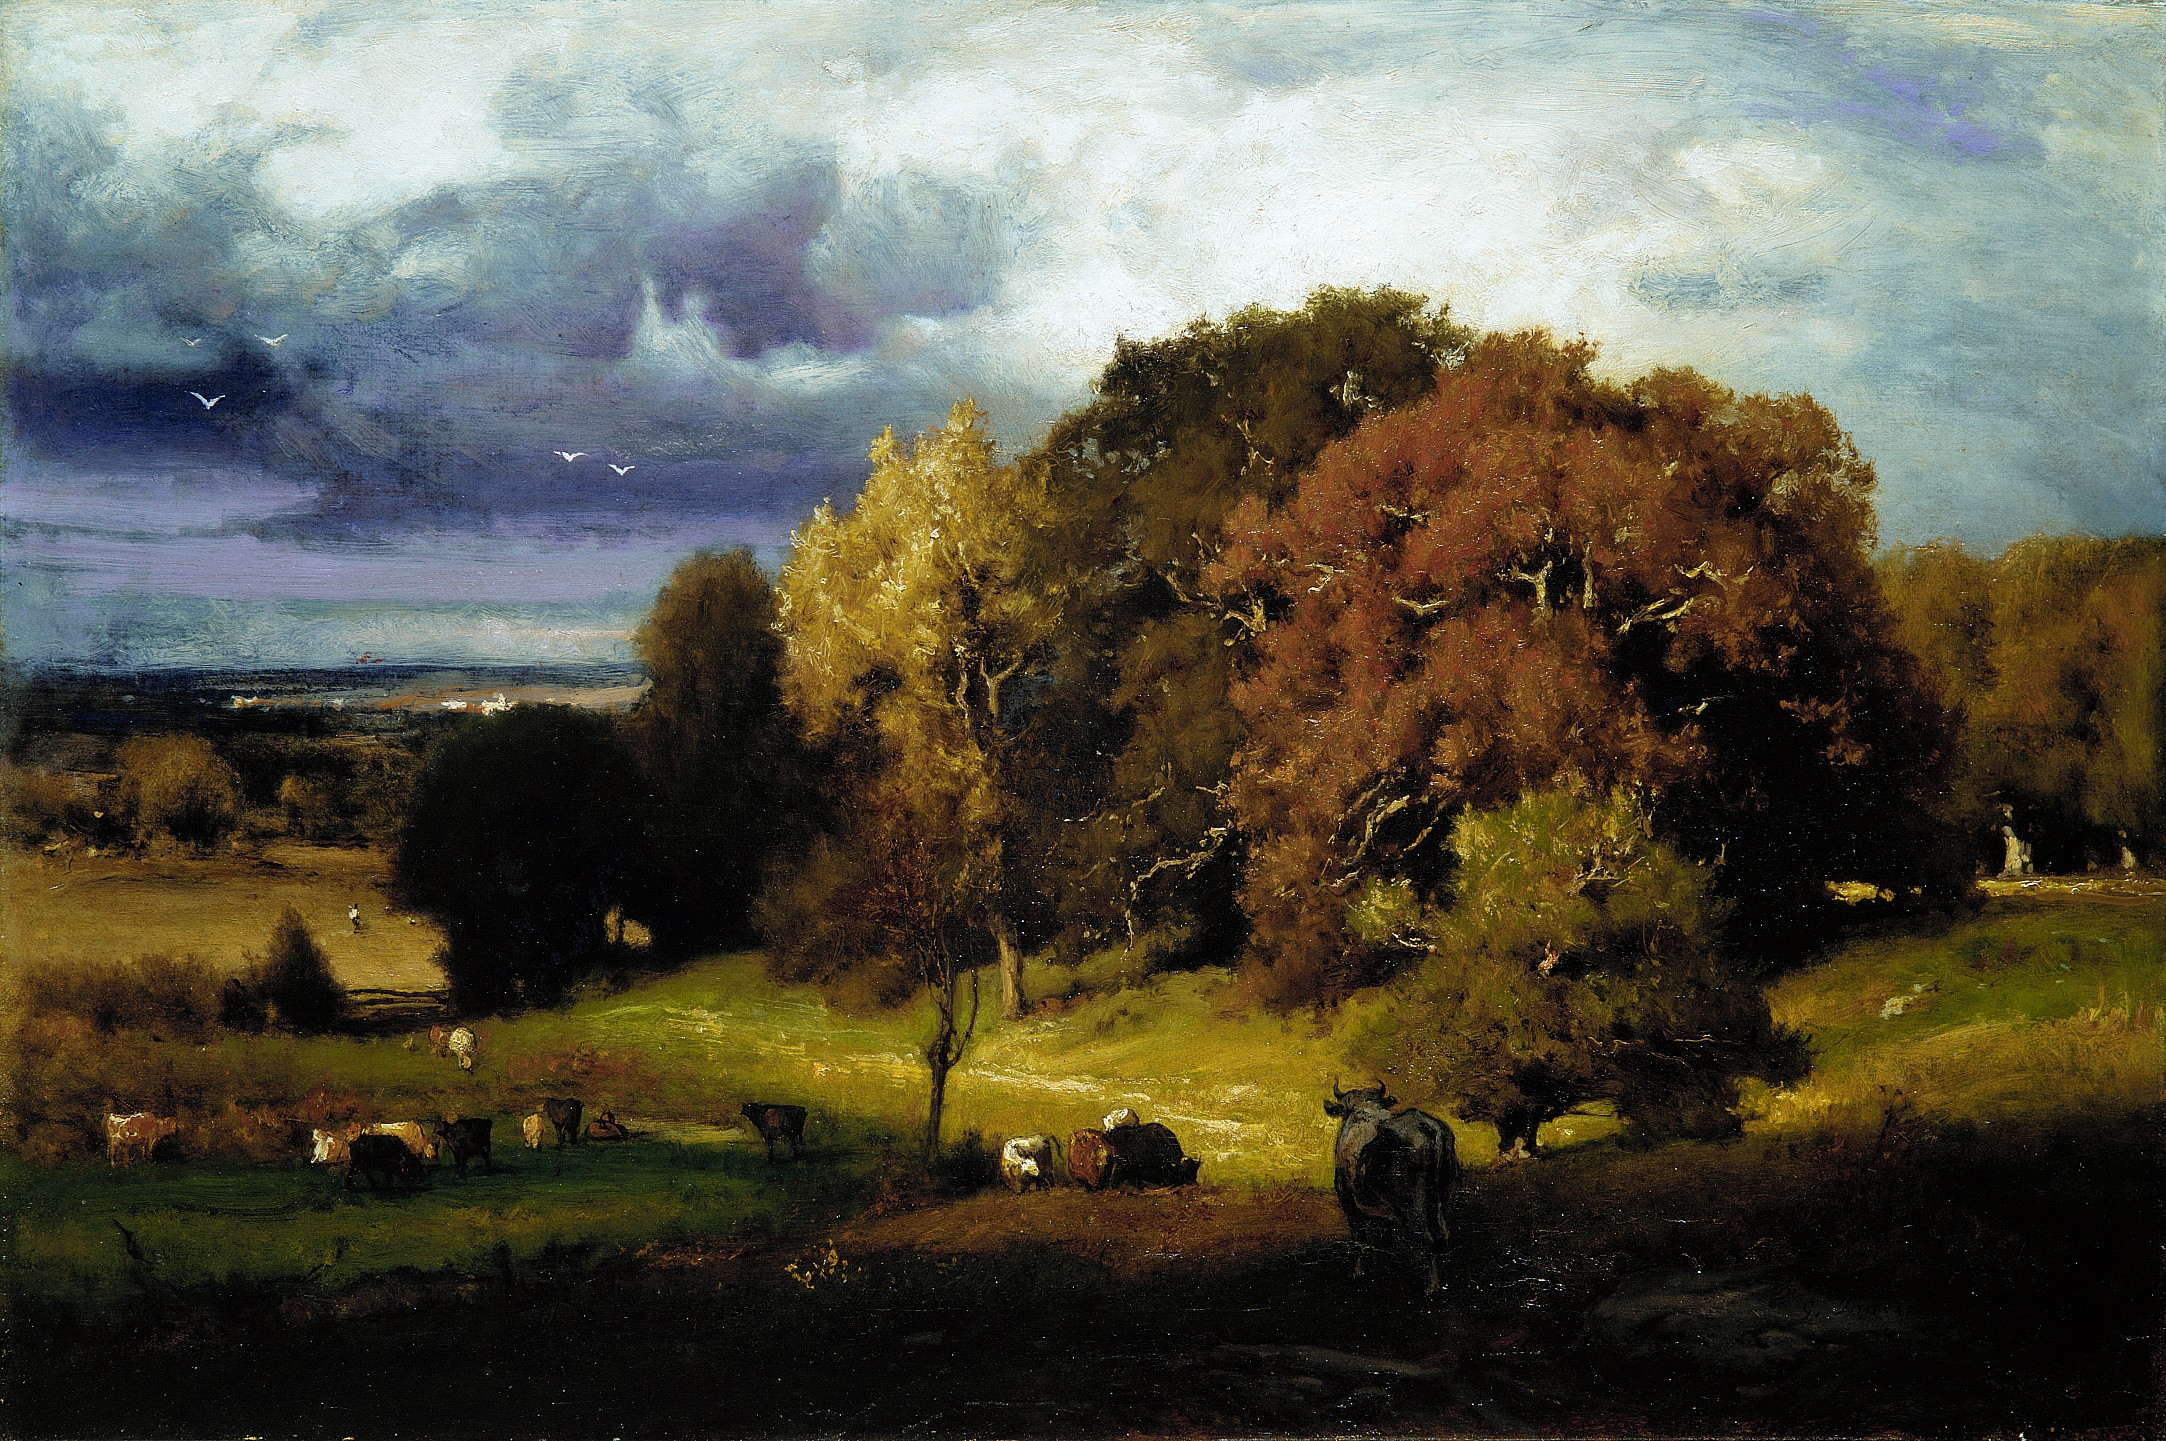
\includegraphics[width=\textwidth]{ForestPaintings/R1innessautumnoaks.jpg}
\end{minipage}
\hfill
\begin{minipage}[b]{.49\textwidth}
	\centering
	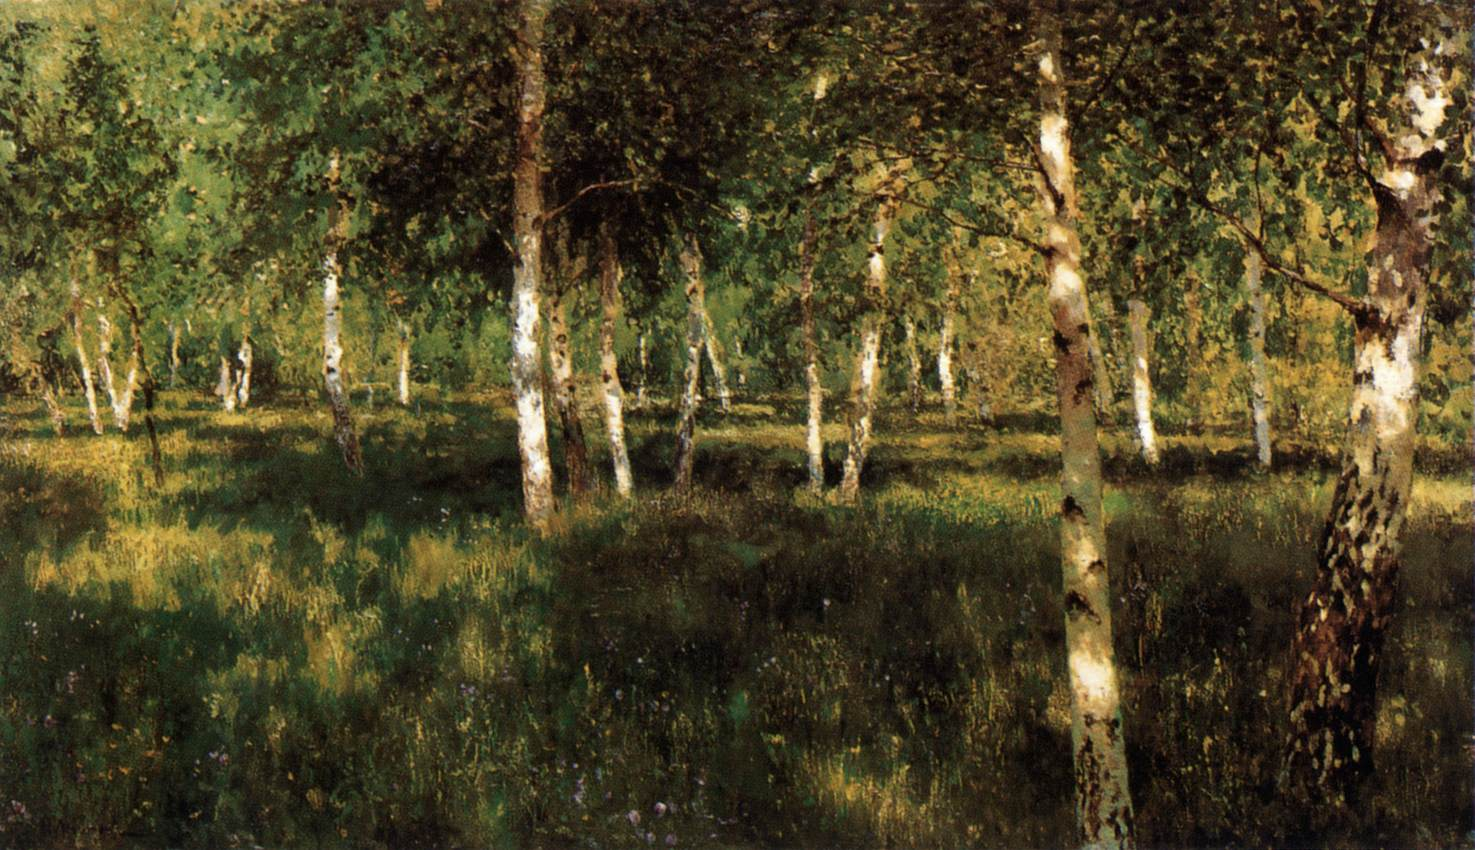
\includegraphics[width=\textwidth]{ForestPaintings/R2levitanbirchgrove.jpg}
\end{minipage}
\begin{minipage}[b]{.49\textwidth}
    \caption{\emph{Autumn Oaks} - George Inness}
\end{minipage}
\begin{minipage}[b]{.49\textwidth}
    \caption{\emph{Birch Grove} - Isaac Levitan}
\end{minipage}
\end{figure}

\subsubsection{Stylized forest paintings}
\begin {figure}[h!]
\centering
\begin{minipage}[b]{.49\textwidth}
	\centering
	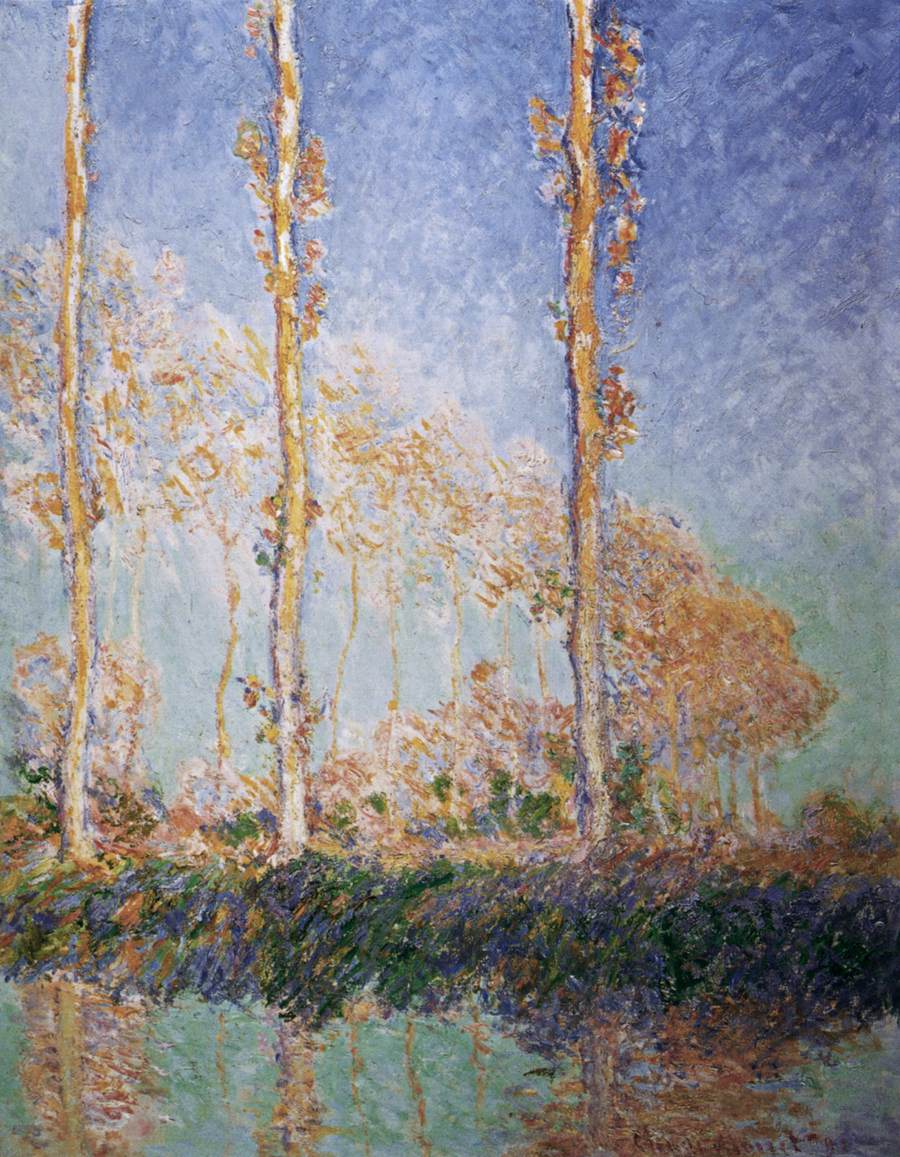
\includegraphics[width=0.9\textwidth]{ForestPaintings/S1monetpoplars.jpg}
\end{minipage}
\hfill
\begin{minipage}[b]{.49\textwidth}
	\centering
	\includegraphics[width=\textwidth]{ForestPaintings/S2hartleyautumncolor.jpg}
\end{minipage}
\begin{minipage}[t]{.49\textwidth}
	\caption{\emph{Poplars} - Claude Monet}
\end{minipage}
\begin{minipage}[t]{.49\textwidth}
	\caption{\emph{Autumn Color} - Marsden Hartley}
\end{minipage}
\end{figure}

\newpage
\subsection{Sea}

\subsubsection{Realistic seascape paintings}
\begin {figure}[h!]
\centering
\begin{minipage}[b]{.49\textwidth}
	\centering
	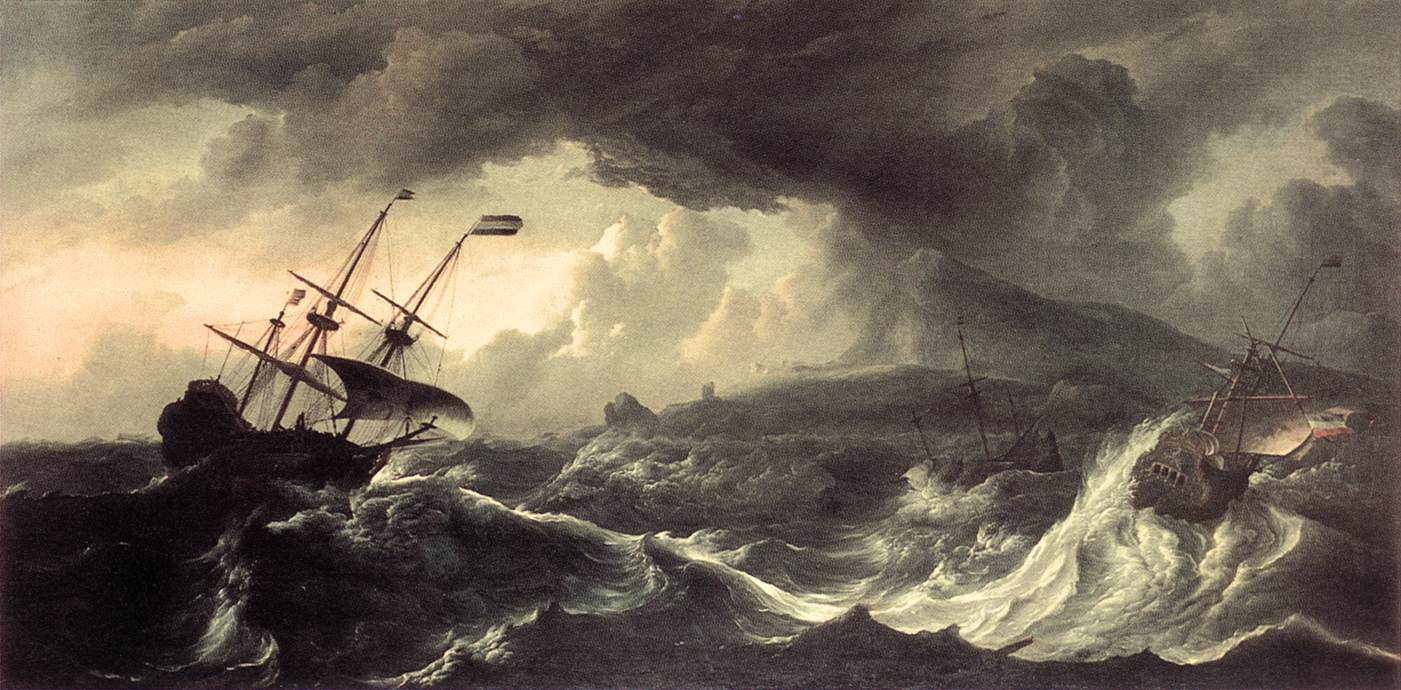
\includegraphics[width=\textwidth]{SeaPaintings/R1backhuysenshipsrunningagroundinastorm.jpg}
    \caption{\emph{Ships Running Aground in a Storm} - Ludolf Backhuysen}
\end{minipage}
\hfill
\begin{minipage}[b]{.49\textwidth}
	\centering
	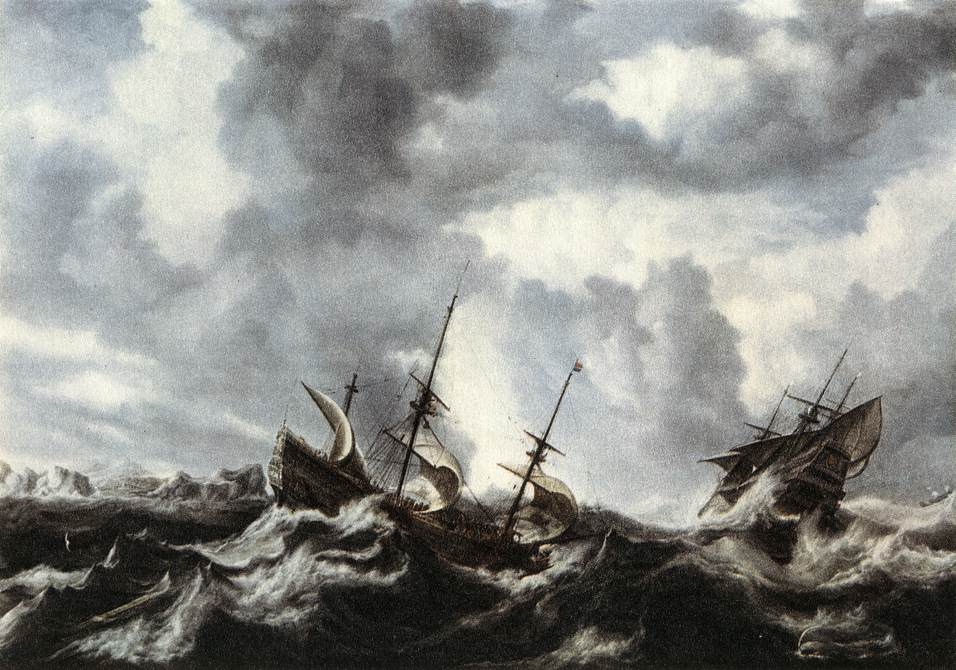
\includegraphics[width=\textwidth]{SeaPaintings/R2peetersstormonthesea.jpg}
    \caption{\emph{Storm on the Sea} - Bonaventura Peeters}
\end{minipage}
\end{figure}

\subsubsection{Stylized seascape paintings}
\begin {figure}[h!]
\centering
\begin{minipage}[b]{.49\textwidth}
	\centering
	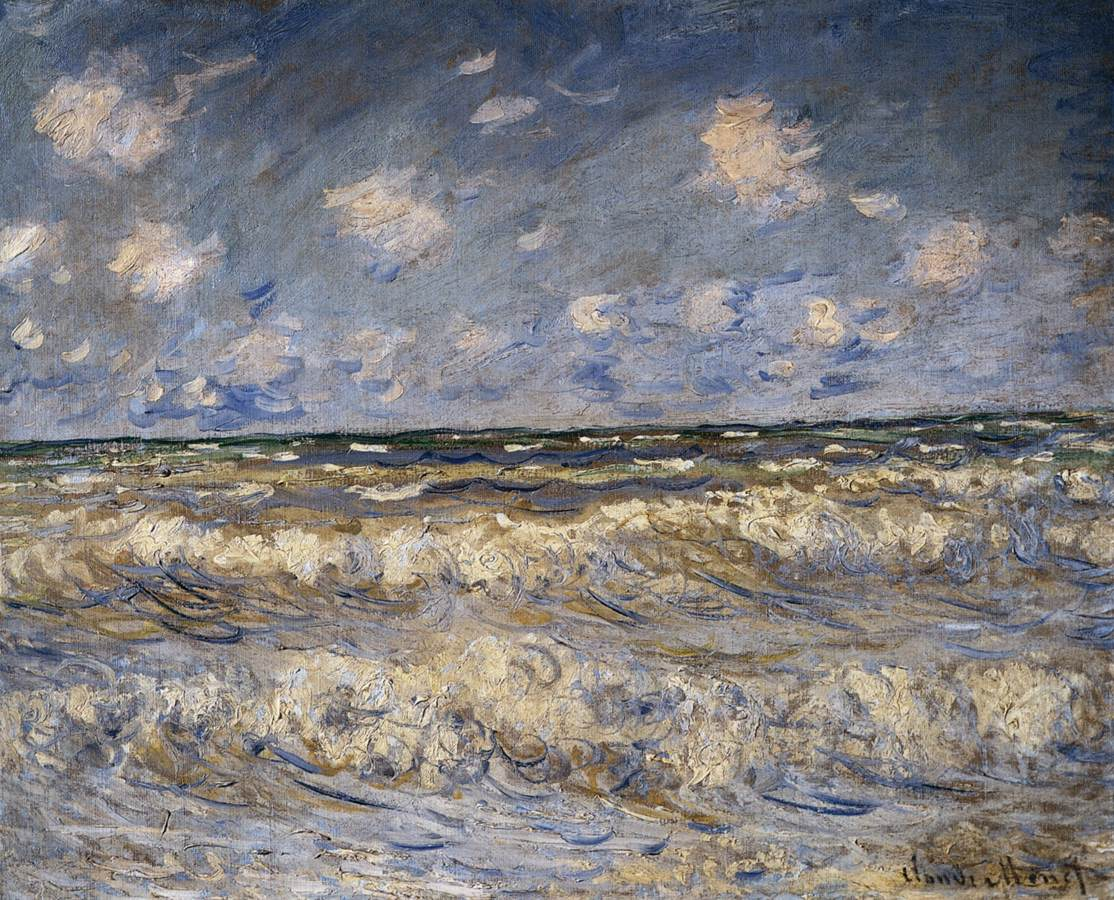
\includegraphics[width=\textwidth]{SeaPaintings/S1monetstormysea.jpg}
	\caption{\emph{Stormy Sea} - Claude Monet}
\end{minipage}
\hfill
\begin{minipage}[b]{.49\textwidth}
	\centering
	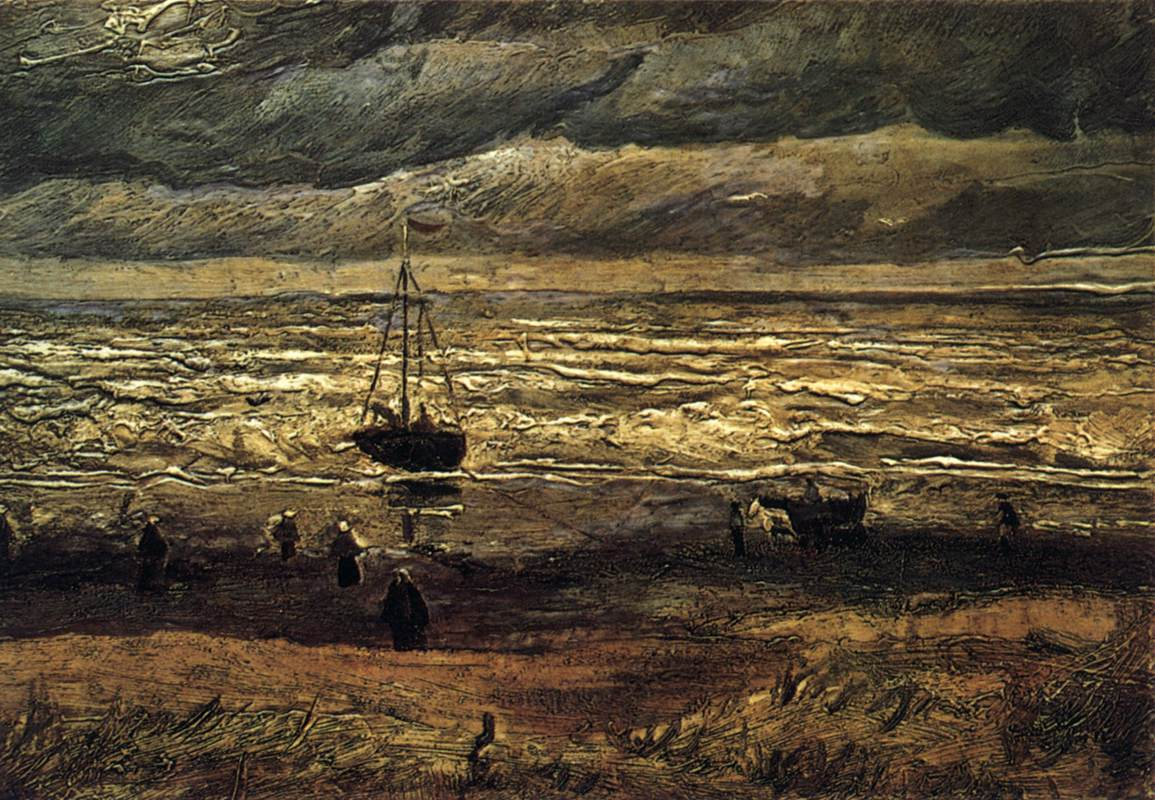
\includegraphics[width=\textwidth]{SeaPaintings/S2vangoghbeachscheveningenstormyweather.jpg}
    \caption{\emph{Beach at Scheveningen in Stormy Weather} - Vincent van Gogh}
\end{minipage}
\end{figure}

\newpage
\subsection{Snow}

\subsubsection{Realistic snow paintings}
\begin {figure}[h!]
\centering
\begin{minipage}[b]{.49\textwidth}
	\centering
	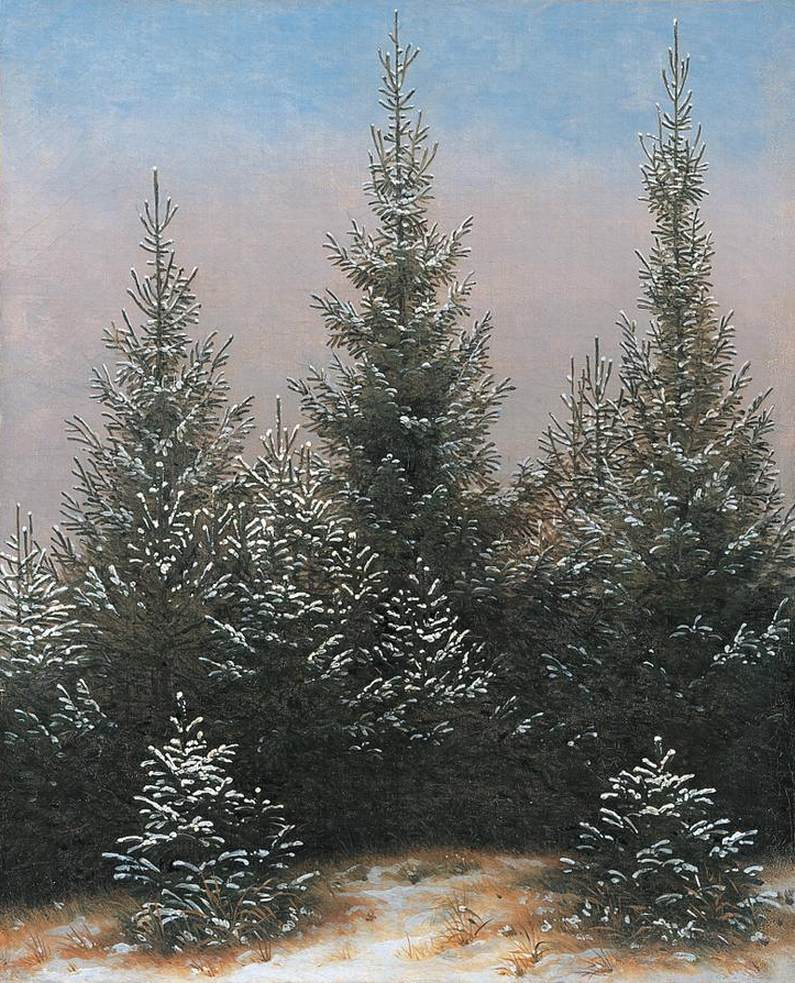
\includegraphics[width=\textwidth]{SnowPaintings/R1friedrichfirtreesinthesnow.jpg}
    \caption{\emph{Fir Trees in the Snow} - Caspar David Friedrich}
\end{minipage}
\hfill
\begin{minipage}[b]{.49\textwidth}
	\centering
	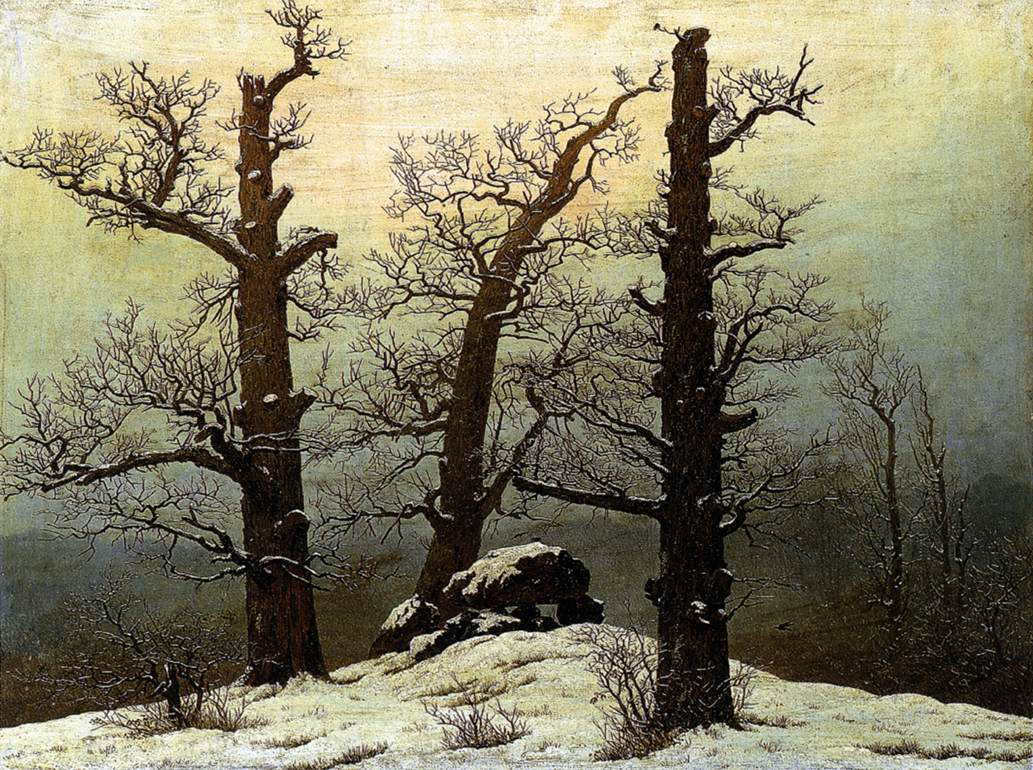
\includegraphics[width=\textwidth]{SnowPaintings/R2friedrichdolmeninthesnow.jpg}
    \caption{\emph{Dolmen in the Snow} - Caspar David Friedrich}
\end{minipage}
\end{figure}

\subsubsection{Stylized snow paintings}
\begin {figure}[h!]
\centering
\begin{minipage}[b]{.49\textwidth}
	\centering
	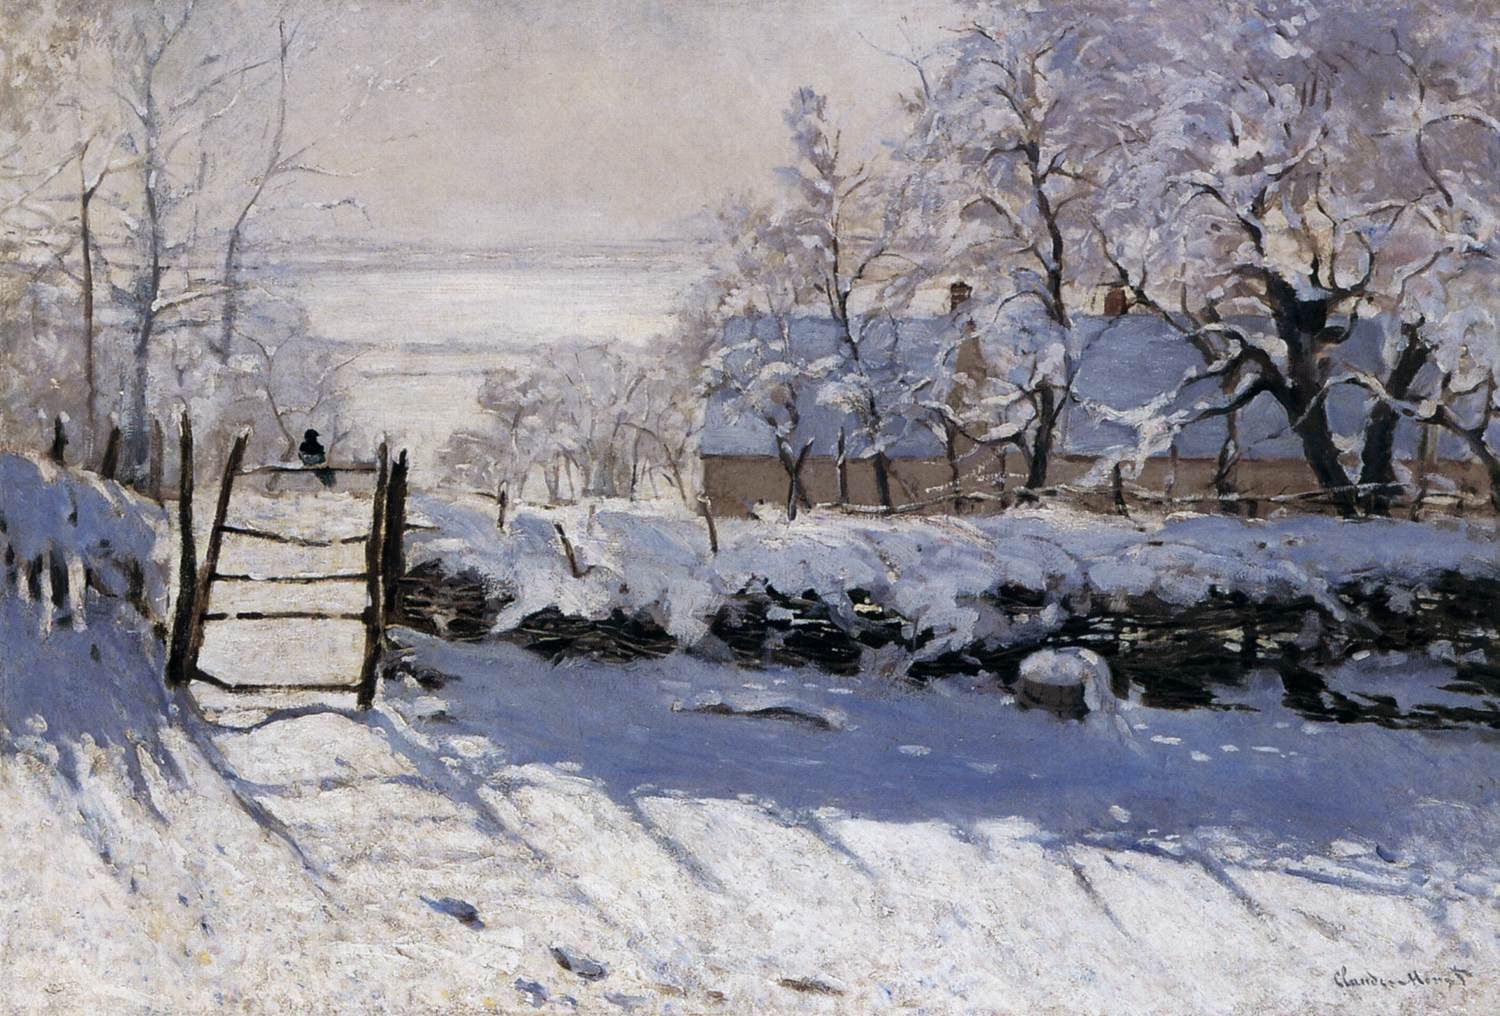
\includegraphics[width=\textwidth]{SnowPaintings/S1monetthemagpie.jpg}
    \caption{\emph{The Magpie} - Claude Monet}
\end{minipage}
\hfill
\begin{minipage}[b]{.49\textwidth}
	\centering
	\includegraphics[width=\textwidth]{SnowPaintings/S2munchtheyellowlog.jpg}
    \caption{\emph{The Yellow Log} - Edvard Munch}
\end{minipage}
\end{figure}


\end{document}